\begin{figure}[]
        \subfloat[The Graph Produced by The Plotting Function using the Euler Method]{
        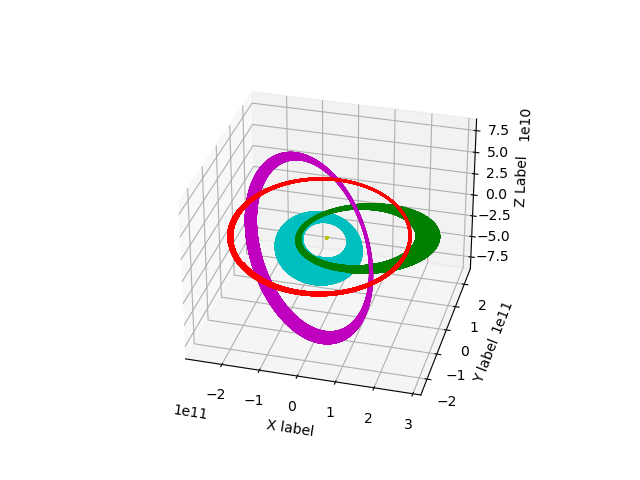
\includegraphics[width=0.5\columnwidth]{Euler Method/Euler Graph.png}}
        \subfloat[The Graph Produced by The Plotting Function using the Euler-Cromer Method]{
        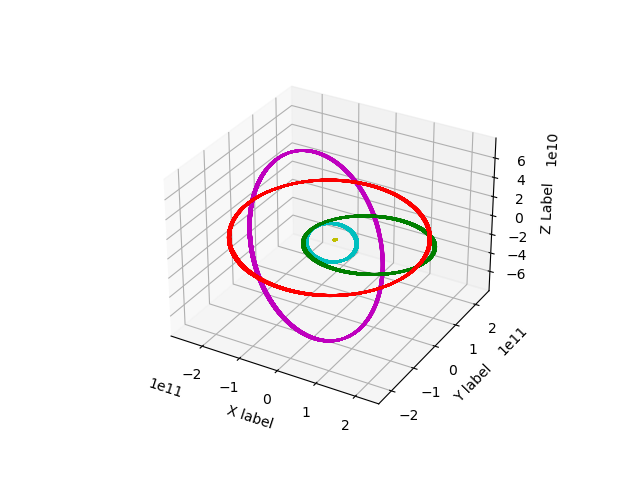
\includegraphics[width=0.5\columnwidth]{Euler-Cromer Method/Euler-Cromer Graph.png}}
        \caption{These plots were produced by the plotting function and are a 3 Dimension rendering of the movement of the bodies as taken in the 3,600-second time steps iterated 100,000 times. The Yellow Dot is a representation of the Sun, The Cyan Ellipse shows the orbit of Mercury, The magenta ellipse shows the orbit of Venus, The Green Ellipse shows the orbit of Earth and the Red ellipse shows the orbit of Mars}
        \label{plot:orbits}
     \end{figure}